\documentclass[a4paper,11pt,fleqn,twoside,openright]{memoir} 	% Openright aabner kapitler paa hoejresider (openany begge)
%%%% PACKAGES %%%%
\usepackage{amsmath}

% ¤¤ Oversaettelse og tegnsaetning ¤¤ %
\usepackage[utf8]{inputenc}					% Input-indkodning af tegnsaet (UTF8)
\usepackage[english]{babel}					% Dokumentets sprog
\usepackage[T1]{fontenc}					% Output-indkodning af tegnsaet (T1)
\usepackage{ragged2e,anyfontsize}			% Justering af elementer
%\usepackage{fixltx2e}						% Retter forskellige fejl i LaTeX-kernen
																			
% ¤¤ Figurer og tabeller (floats) ¤¤ %
\usepackage{graphicx} 						% Haandtering af eksterne billeder (JPG, PNG, PDF)
\usepackage{adjustbox}
\usepackage{multirow}                		% Fletning af raekker og kolonner (\multicolumn og \multirow)
\usepackage{colortbl} 						% Farver i tabeller (fx \columncolor, \rowcolor og \cellcolor)
\usepackage[dvipsnames,table,xcdraw]{xcolor}				% Definer farver med \definecolor. Se mere: http://en.wikibooks.org/wiki/LaTeX/Colors
%\usepackage{flafter}						% Soerger for at floats ikke optraeder i teksten foer deres reference
%\let\newfloat\relax 						% Justering mellem float-pakken og memoir
\usepackage{float}							% Muliggoer eksakt placering af floats, f.eks. \begin{figure}[H]
\usepackage{eso-pic}						% Tilfoej billedekommandoer paa hver side
\usepackage{wrapfig}						% Indsaettelse af figurer omsvoebt af tekst. \begin{wrapfigure}{Placering}{Stoerrelse}
\usepackage{multicol}         	        	% Muliggoer tekst i spalter
\usepackage{rotating}						% Rotation af tekst med \begin{sideways}...\end{sideways}

% ¤¤ Matematik mm. ¤¤
\usepackage{amsmath,amssymb,stmaryrd} 		% Avancerede matematik-udvidelser
\usepackage{mathtools}						% Andre matematik- og tegnudvidelser
\usepackage{textcomp}                 		% Symbol-udvidelser (f.eks. promille-tegn med \textperthousand )
\usepackage{siunitx}						% Flot og konsistent praesentation af tal og enheder med \si{enhed} og \SI{tal}{enhed}
\sisetup{output-decimal-marker = {,}}		% Opsaetning af \SI (DE for komma som decimalseparator) 
\usepackage[version=3]{mhchem} 				% Kemi-pakke til flot og let notation af formler, f.eks. \ce{Fe2O3}
%\usepackage{rsphrase}						% Kemi-pakke til RS-saetninger, f.eks. \rsphrase{R1}

% ¤¤ Referencer og kilder ¤¤ %
\usepackage[english]{varioref}				% Muliggoer bl.a. krydshenvisninger med sidetal (\vref)
%\usepackage{natbib}							% Udvidelse med naturvidenskabelige citationsmodeller
%\usepackage{xr}							% Referencer til eksternt dokument med \externaldocument{<NAVN>}
%\usepackage{glossaries}					% Terminologi- eller symbolliste (se mere i Daleifs Latex-bog)

% ¤¤ Misc. ¤¤ %
\usepackage{listings}						% Placer kildekode i dokumentet med \begin{lstlisting}...\end{lstlisting}
\usepackage{lipsum}							% Dummy text \lipsum[..]
\usepackage{enumitem}			% Muliggoer enkelt konfiguration af lister
\usepackage{pdfpages}						% Goer det muligt at inkludere pdf-dokumenter med kommandoen \includepdf[pages={x-y}]{fil.pdf}	
\pdfoptionpdfminorversion=6					% Muliggoer inkludering af pdf dokumenter, af version 1.6 og hoejere
\pretolerance=2500 							% Justering af afstand mellem ord (hoejt tal, mindre orddeling og mere luft mellem ord)

% Kommentarer og rettelser med \fxnote. Med 'final' i stedet for 'draft' udloeser hver note en error i den faerdige rapport.
\usepackage[footnote,draft,english,silent,nomargin]{fixme}		
%% brugt til at skrive tale transcripts%%

%%%% CUSTOM SETTINGS %%%%

% ¤¤ Marginer ¤¤ %
\setlrmarginsandblock{3.5cm}{2.5cm}{*}		% \setlrmarginsandblock{Indbinding}{Kant}{Ratio}
\setulmarginsandblock{2.5cm}{3.0cm}{*}		% \setulmarginsandblock{Top}{Bund}{Ratio}
\checkandfixthelayout 						% Oversaetter vaerdier til brug for andre pakker

%	¤¤ Afsnitsformatering ¤¤ %
\setlength{\parindent}{0mm}           		% Stoerrelse af indryk
\setlength{\parskip}{3mm}          			% Afstand mellem afsnit ved brug af double Enter
\linespread{1,1}							% Linie afstand

% ¤¤ Litteraturlisten ¤¤ %
%\bibpunct[,]{[}{]}{;}{a}{,}{,} 				% Definerer de 6 parametre ved Harvard henvisning (bl.a. parantestype og seperatortegn)
\bibliographystyle{ieeetr}			% Udseende af litteraturlisten. %abbrv

%\usepackage[sorting=none,firstinits=true]{biblatex}

%\bibliographystyle{unsrtnat}

% ¤¤ Indholdsfortegnelse ¤¤ %
\setsecnumdepth{subsection}		 			% Dybden af nummerede overkrifter (part/chapter/section/subsection)
\maxsecnumdepth{subsection}					% Dokumentklassens graense for nummereringsdybde
\settocdepth{subsection} 					% Dybden af indholdsfortegnelsen

% ¤¤ Lister ¤¤ %
\setlist{
  topsep=0pt,								% Vertikal afstand mellem tekst og listen
  itemsep=-1ex,								% Vertikal afstand mellem items
} 

% ¤¤ Visuelle referencer ¤¤ %
\usepackage[colorlinks]{hyperref}			% Danner klikbare referencer (hyperlinks) i dokumentet.
\hypersetup{colorlinks = true,				% Opsaetning af farvede hyperlinks (interne links, citeringer og URL)
    linkcolor = black,
    citecolor = black,
    urlcolor = black
}

% ¤¤ Opsaetning af figur- og tabeltekst ¤¤ %
\captionnamefont{\small\bfseries\itshape}	% Opsaetning af tekstdelen ('Figur' eller 'Tabel')
\captiontitlefont{\small}					% Opsaetning af nummerering
\captiondelim{. }							% Seperator mellem nummerering og figurtekst
\hangcaption								% Venstrejusterer flere-liniers figurtekst under hinanden
\captionwidth{\linewidth}					% Bredden af figurteksten
\setlength{\belowcaptionskip}{0pt}			% Afstand under figurteksten
		
% ¤¤ Opsaetning af listings ¤¤ %
\definecolor{commentGreen}{RGB}{34,139,24}
\definecolor{stringPurple}{RGB}{208,76,239}

\lstset{language=Matlab,					% Sprog
	basicstyle=\ttfamily\scriptsize,		% Opsaetning af teksten
	keywords={for,if,while,else,elseif,		% Noegleord at fremhaeve
			  end,break,return,case,
			  switch,function},
	keywordstyle=\color{blue},				% Opsaetning af noegleord
	commentstyle=\color{commentGreen},		% Opsaetning af kommentarer
	stringstyle=\color{stringPurple},		% Opsaetning af strenge
	showstringspaces=false,					% Mellemrum i strenge enten vist eller blanke
	numbers=left, numberstyle=\tiny,		% Linjenumre
	extendedchars=true, 					% Tillader specielle karakterer
	columns=flexible,						% Kolonnejustering
	breaklines, breakatwhitespace=true,		% Bryd lange linjer
}

% ¤¤ Navngivning ¤¤ %
\addto\captionsdanish{
	\renewcommand\appendixname{Appendiks}
	\renewcommand\contentsname{Indholdsfortegnelse}	
	\renewcommand\appendixpagename{Appendiks}
	\renewcommand\appendixtocname{Appendiks}
	\renewcommand\cftchaptername{\chaptername~}				% Skriver "Kapitel" foran kapitlerne i indholdsfortegnelsen
	\renewcommand\cftappendixname{\appendixname~}			% Skriver "Appendiks" foran appendiks i indholdsfortegnelsen
}

% ¤¤ Kapiteludssende ¤¤ %
\definecolor{numbercolor}{gray}{0.7}		% Definerer en farve til brug til kapiteludseende
\newif\ifchapternonum

\makechapterstyle{jenor}{					% Definerer kapiteludseende frem til ...
  \renewcommand\beforechapskip{0pt}
  \renewcommand\printchaptername{}
  \renewcommand\printchapternum{}
  \renewcommand\printchapternonum{\chapternonumtrue}
  \renewcommand\chaptitlefont{\fontfamily{pbk}\fontseries{db}\fontshape{n}\fontsize{25}{35}\selectfont\raggedleft}
  \renewcommand\chapnumfont{\fontfamily{pbk}\fontseries{m}\fontshape{n}\fontsize{1in}{0in}\selectfont\color{numbercolor}}
  \renewcommand\printchaptertitle[1]{%
    \noindent
    \ifchapternonum
    \begin{tabularx}{\textwidth}{X}
    {\let\\\newline\chaptitlefont ##1\par} 
    \end{tabularx}
    \par\vskip-2.5mm\hrule
    \else
    \begin{tabularx}{\textwidth}{Xl}
    {\parbox[b]{\linewidth}{\chaptitlefont ##1}} & \raisebox{-15pt}{\chapnumfont \thechapter}
    \end{tabularx}
    \par\vskip2mm\hrule
    \fi
  }
}											% ... her

\chapterstyle{jenor}						% Valg af kapiteludseende - Google 'memoir chapter styles' for alternativer

% ¤¤ Sidehoved ¤¤ %

\makepagestyle{Uni}							% Definerer sidehoved og sidefod udseende frem til ...
\makepsmarks{Uni}{%
	\createmark{chapter}{left}{shownumber}{}{. \ }
	\createmark{section}{right}{shownumber}{}{. \ }
	\createplainmark{toc}{both}{\contentsname}
	\createplainmark{lof}{both}{\listfigurename}
	\createplainmark{lot}{both}{\listtablename}
	\createplainmark{bib}{both}{\bibname}
	\createplainmark{index}{both}{\indexname}
	\createplainmark{glossary}{both}{\glossaryname}
}
\nouppercaseheads											% Ingen Caps oenskes

\makeevenhead{Uni}{Group DS303E16}{}{\leftmark}				% Definerer lige siders sidehoved (\makeevenhead{Navn}{Venstre}{Center}{Hoejre})
\makeoddhead{Uni}{\rightmark}{}{Aalborg University}			% Definerer ulige siders sidehoved (\makeoddhead{Navn}{Venstre}{Center}{Hoejre})
\makeevenfoot{Uni}{\thepage}{}{}							% Definerer lige siders sidefod (\makeevenfoot{Navn}{Venstre}{Center}{Hoejre})
\makeoddfoot{Uni}{}{}{\thepage}								% Definerer ulige siders sidefod (\makeoddfoot{Navn}{Venstre}{Center}{Hoejre})
\makeheadrule{Uni}{\textwidth}{0.5pt}						% Tilfoejer en streg under sidehovedets indhold
\makefootrule{Uni}{\textwidth}{0.5pt}{1mm}					% Tilfoejer en streg under sidefodens indhold

\copypagestyle{Unichap}{Uni}								% Sidehoved for kapitelsider defineres som standardsider, men med blank sidehoved
\makeoddhead{Unichap}{}{}{}
\makeevenhead{Unichap}{}{}{}
\makeheadrule{Unichap}{\textwidth}{0pt}
\aliaspagestyle{chapter}{Unichap}							% Den ny style vaelges til at gaelde for chapters
															% ... her
															
\pagestyle{Uni}												% Valg af sidehoved og sidefod (benyt "plain" for ingen sidehoved/fod)


%%%% CUSTOM COMMANDS %%%%

% ¤¤ Specielle tegn ¤¤ %
\newcommand{\decC}{^{\circ}\text{C}}
\newcommand{\dec}{^{\circ}}
\newcommand{\m}{\cdot}


%%%% ORDDELING %%%%

\hyphenation{}

%C# format
\usepackage[T1]{fontenc}
\usepackage[scaled]{beramono}

\usepackage{color}
\definecolor{bluekeywords}{rgb}{0.13,0.13,1}
\definecolor{greencomments}{rgb}{0,0.5,0}
\definecolor{redstrings}{rgb}{0.9,0,0}

\lstset{language=[Sharp]C,
captionpos=b,
numbers=left, %Nummerierung
numberstyle=\tiny, % kleine Zeilennummern
frame=lines, % Oberhalb und unterhalb des Listings ist eine Linie
showspaces=false,
showtabs=false,
breaklines=true,
showstringspaces=false,
breakatwhitespace=true,
escapeinside={(*@}{@*)},
commentstyle=\color{greencomments},
morekeywords={partial, var, value, get, set},
keywordstyle=\color{bluekeywords},
stringstyle=\color{redstrings},
basicstyle=\ttfamily\small,
}
\renewcommand\lstlistingname{Code fragment}


\usepackage{blindtext}
\usepackage{scrextend}
\addtokomafont{labelinglabel}{\sffamily}
%% Extra ting som vi selv har sat på.
\usepackage{xargs}
\usepackage[colorinlistoftodos,prependcaption,textsize=tiny]{todonotes}
\newcommandx{\unsure}[2][1=]{\todo[linecolor=red,backgroundcolor=red!25,bordercolor=red,#1]{#2}}
\newcommandx{\change}[2][1=]{\todo[linecolor=blue,backgroundcolor=blue!25,bordercolor=blue,#1]{#2}}
\newcommandx{\info}[2][1=]{\todo[linecolor=OliveGreen,backgroundcolor=OliveGreen!25,bordercolor=OliveGreen,#1]{#2}}
\newcommandx{\improvement}[2][1=]{\todo[linecolor=Plum,backgroundcolor=Plum!25,bordercolor=Plum,#1]{#2}}
\usepackage{longtable}
%% Get superscript style citations with square brackets
\usepackage[super]{natbib}
\setcitestyle{square}
\raggedbottom

\begin{document}

\frontmatter

\thispagestyle{empty}
\begin{center}
\vspace{3cm}

\phantom{hul}

\phantom{hul}

\phantom{hul}

\textsl{\Huge Centralization of farming information} \\ \vspace{1cm}

\rule{13cm}{3mm} \\ \vspace{1.5cm}
\vspace{1cm}

%\includegraphics[width=0.8\textwidth]{images/frontpage.png}

\vspace{2cm} 
\textsc{\Large P3-project \\
Group DS303E16 \\
Software\\
Aalborg University\\Dec 21, 2016\\}
\end{center}

\cleardoublepage
\phantomsection
\pdfbookmark[0]{Titlesheet}{titlesheet}
\thispagestyle{empty}

\begin{minipage}[t]{0.48\textwidth}
\vspace*{-25pt}			%\vspace*{-9pt}

\includegraphics[height=4cm]{images/AAU-logo-stud-UK-RGB}
\end{minipage}
\hfill
\begin{minipage}[t]{0.48\textwidth}
{\small \textbf{Department of Computer Science}\\
\small Salma LagerLöfsvej 300 \\
\small Phone: +45 99 40 99 40 \\
\small Fax: +45 99 40 97 98 \\
\small http://www.cs.aau.dk}

\end{minipage}

\vspace*{1cm}

\begin{minipage}[t]{0.48\textwidth}
\textbf{Title:} \\[5pt]\bigskip\hspace{2ex}
PLACEHOLDER TITLE

\textbf{Project:} \\[5pt]\bigskip\hspace{2ex}
P3-project

\textbf{Project period:} \\[5pt]\bigskip\hspace{2ex}
September 2016 - December 2016

\textbf{Project group:} \\[5pt]\bigskip\hspace{2ex}
DS303E16

\textbf{Authors:} \\[5pt]\hspace*{2ex}
Alexander E. S. Ostenfeld \\\hspace*{2ex}
Asger Gitz-Johansen \\\hspace*{2ex}
Anonym Dværgkanin \\\hspace*{2ex} \todo{FIX NAVN FØR AFLEVERING!}
Martin Fabrin Karkov \\\hspace*{2ex}
Mikkel Elkjær Holm \\\hspace*{2ex}
Rasmus Jespersen \\\bigskip\hspace*{2ex}
Tobias Klitgaard Sørensen

\textbf{Supervisor:} \\[5pt]\hspace*{2ex}
Muhammad Aamir Saleem

\vspace*{1cm}

%\textbf{Oplagstal: TODO} \\
\textbf{Pagecount: ???} \\
%\textbf{Appendix: TODO} \\ 
\textbf{Finished 2016-12-21}

\end{minipage}
\hfill
\begin{minipage}[t]{0.483\textwidth}
Abstract: \\[5pt]
\fbox{\parbox{7cm}{\bigskip\input{formalia/abstract}\bigskip}}
\end{minipage}

\vfill

{\footnotesize\itshape The content of the report is freely available, but publication (with source reference) may only take place in agreement with the authors.}

% Rapportens indhold er frit tilgængeligt, men offentliggørelse (med kildeangivelse) må kun ske efter aftale med forfatterne.
% The content of the report is freely available, but publication (with source reference) may only take place in agreement with the authors.
\cleardoublepage

\chapter*{Preface}
\include{formalia/preface}

\cleardoublepage

\phantomsection
\pdfbookmark[0]{Contents}{contents}
\tableofcontents*

\mainmatter
%%% MAIN REPORT %%%

%% Introduction %%
\chapter{Project description}
In this chapter we will describe what is required of the report and program, what methods have been used to evaluate and delineate the interested parties and methods used in program development. 

\section{Purpose}
The third semester of the software bachelor at AAU, has a curriculum that aims to express the purpose of the P3-project and therefore this report.

The purpose being:
\begin{quotation}
Den studerende skal opnå viden om problemstillinger og fundamentale teknikker i udvikling af applikationer til løsning af realistiske opgaver; og opnå erfaring med udvikling af store systemer, arbejdsdeling og kvalitetskontrol herunder aftestning og afprøvning.
\end{quotation}

Translated:
\begin{quotation}
The student must acquire knowledge about problems and fundamental techniques in the development of applications in the pursuit of solving realistic problems; and acquire experience in developing large systems, work distribution and quality control including trial and testing.
\end{quotation}

In parallel with the P3-project, courses in Systems Development, Algorithms and Datastructures and Design and Evaluation of User Interfaces were held. We will use the knowledge gained from these courses to enhance and ensure the quality of the report and subsequent program.

A requirement for this project is that we, as a group, work together with, and develop a solution for, a user and describe the essential parts of the process.


\section{Methods}
\input{intro/description/methods.tex}

\part{Background}
\chapter{Introduction}
\todo{HC: Fix typeface så square-brackets ikke ligner math mode.}






%% hej champ! skriv lige baggrunden for projectet, og projekt beskrivelsen i "intro/description/purpose" det gør det lidt nemmere at sætte op når det er. :) og stop venligst med at bruge sections.

%først overall area, så problem area og så det område vi specific ønsker %at arbejde med.


%% farmers what do they do.
%% stats on farmers
%% they are important





%\section{Introduction}
\todo{skrive lige hele introduktionen på et tidspunkt.}
\todo{Beskriv hvem vi arbejder sammen med og hvorfor.}
\todo{Lav sektion til initierende problem.}
\todo{Initierende problem opdateres løbende.}
"How can we make the information about farming, machines and resources more centrally accesible and have an easy overview as user friendly for the farmer and others in the business."

following initial problem statement:\newline

\begin{center}
"How can we make the information about farming, machines and resources more centrally accesible and have an easy overview as user friendly for the farmer and others in the business."
\end{center}

%% ANALYSIS SPACE %%
\part{Social and Environmental context}

%% PACT-Analyse %%
\chapter{PACT}
\section{People}
\begin{wrapfigure}{R}{0.3\textwidth}
\centering
\vspace{-50pt}

\includegraphics[width=0.3\textwidth, keepaspectratio]{images/pact/people}
\caption{\label{fig:people}Hypothetical group of users.}
\vspace{-50pt}
\end{wrapfigure}
We will here make a short list of the different kinds of peoples in our target audience, and list some of the strengths and weaknesses and unique characteristics. 

\subsection{Independent Farmers}
\begin{wrapfigure}{R}{0.3\textwidth}
\centering
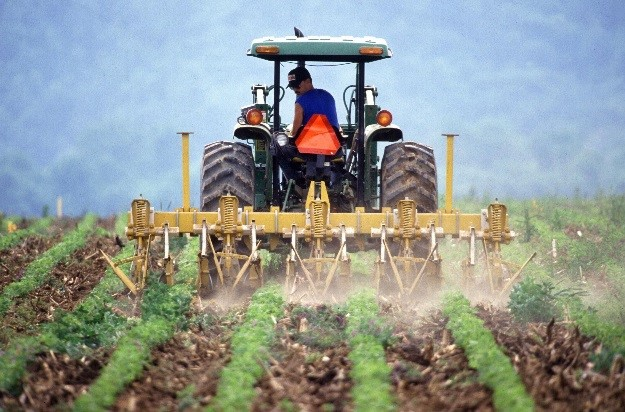
\includegraphics[width=0.3\textwidth, keepaspectratio]{images/pact/tractor}
\caption{\label{fig:independantfarmers}Picture of an independent farmer plowing a field.}
\vspace{-40pt}
\end{wrapfigure}
Independent Farmers need a way to keep track of recourse use of a particular field, and need to know the workload of the field as well. Farmers usually have a passing knowledge of new technology but is sometimes lacking in the application of those technologies.

\subsection{Organized farmers}
Organized farmers such as the company Arla have the same need as the independent farmer to keep track of either a single field of land or a whole slew of plots. Companies usually strife for profit maximization and minimal resource use. They are usually quick to apply new technology for that goal, and have organized rollout of those new technologies.

\subsection{Machinery contractors}
%\begin{wrapfigure}{R}{0.3\textwidth}
%\centering
%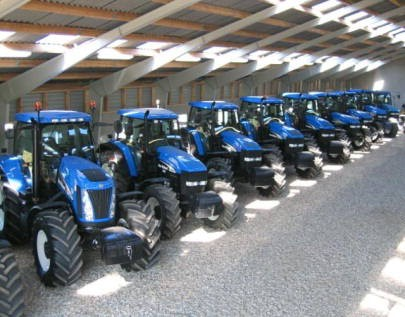
\includegraphics[width=0.3\textwidth, keepaspectratio]{images/pact/lotsoftractors}
%\caption{\label{fig:machinerycontractors}Picture of multiple tractors.}
%\end{wrapfigure}
Machinery contractors are companies that either rent out farm vehicles such as combines, or rent out the service wholesale where a famer rent the contractor to harvest a field for him. The contractors are interested in knowing how many resources a particular field need. This is so that they can help their customers’ needs and to find the right price. 

\section{Activities}
\begin{wrapfigure}{R}{0.3\textwidth}
\centering
\vspace{-10pt}
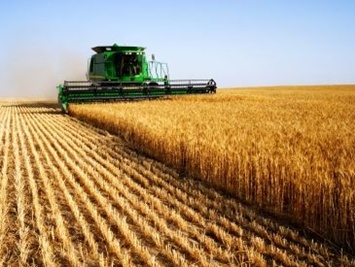
\includegraphics[width=0.3\textwidth, keepaspectratio]{images/pact/hoste}
\caption{\label{fig:activities}Picture of a combine harvester harvesting a field.}
\vspace{-10pt}
\end{wrapfigure}
In this chapter  the constraints and possibilities of the activity are presented, we are doing this to get a better overview of exactly this.
The purpose of the activity is to gain some form of overview of the resource usage when doing some form of work on a field.  This activity will happen ca. 4 times per field per year, which makes it somewhat frequent for some users and very infrequent for other users, relying on the amount of fields that the user interacts with. The activities are time sensitive, meaning you lose much of your produce if any of the tasks happen at a incorrect time. This time sensitivity may make the users more irritable due to the pressure they are under when doing the tasks. Due to this plausible irritability it should be easy to edit the input data, in case of any mistakes. This will be a abstract task that will require a user-friendly design, for proper usage. The input will be a considerable amount of data, which makes some form of keyboard almost required . 

\section{Context}
Intro shit
\subsection{Physical}
In regards to physical constraints that the application might have, we have to consider a quite important aspect: Whether the application is run on a non-static portable device like a touch tablet or smartphone, or if it's run on a personal computer in the users own home office. If the application is portable there is a lot of physical issues that derives from the medium itself, such as:
\begin{itemize}[noitemsep]
    \item Rain, sun glare heavy wind or other external weather hazards that might damage or destroy the device on which the program is being executed.
    \item Distracting the user while driving or doing other important tasks that will require attention.
    \item Power issues and Internet access out on the field.
    \item If the application is being used on a home PC, there is much less issues with Weather and distractions, but the user might want to use the application while his/her memory is fresh.
\end{itemize}

\subsection{Social}
The farmer needs to learn to use the program, before he can draw advantage from it. The user might not have great IT-skills, so the learning curve should be gentle.

\subsection{Organisational}
\begin{itemize}[noitemsep]
    \item The program will enable the user to maximize profits, while minimizing expenses to hiring help, because an estimate for the amount of work required will be available way before it is needed, and therefore give the opportunity to optimize the hiring procedure.
    \item The program will also enable the user to get a better overview of the economy of his field(s), because he will be able to estimate expenses on each field separately and decide if the current approach is sufficiently profitable.
    \item Savings will be possible when buying crops and equipment, because the user will be able to find offers in advance, instead of having to find something in the last minute, during the harvest/sowing/plowing period.
\end{itemize}

\section{Technologies}
Here we will examine the complete technologies of the tablet.

\begin{wrapfigure}{R}{0.3\textwidth}
\centering

\includegraphics[width=0.3\textwidth, keepaspectratio]{images/pact/tablet}
\caption{\label{fig:technologies}Picture of a tablet, which might run the application.}
\end{wrapfigure}
\begin{itemize}[noitemsep]
    \item Bluetooth capabilities
    \item Wireless internet 
    \item Camera
    \item GPS
    \item Timer 
    \item Clock 
    \item Flashlight 
    \item Storage of digital information 
    \item Loudspeakers 
    \item Touchscreen
    \item Digital games 
    \item Personal assistant (digital)
    \item Accelerometer
    \item GSM, HDSPA, LTE (cellular network)
    \item NFC (near field communication)
\end{itemize}

\subsection{Input}
The input of the tablet is primarily its touchscreen and the physical buttons placed on the device such as the on/off button or the volume. Secondary the input of the tablet is the voice controlled command the newer models supports. Some model of the tablet also have a small keyboard for input.

\subsection{Output}
The output of the average tablet is the tablets display/screen where it is possible for the tablet to show the user a wide array of different information. The output would also be sound as all tablets have a set of loudspeakers embedded in them or, at the very least, an audio jack. Sound could fx be used for encouragement for the user to pay attention to the device. 

\subsection{Communication}
The possibilities of communication in a tablet is Wi-Fi, Bluetooth, mobile data connection and NFC. These can be used to communicate data to an offsite server or communicate with other users. The GPS can be used to communicate the location of the user or equipment to a tracking system.


%% SOLUTION SPACE %%
\part{Solution} % placeholder navn

\chapter{Design}
%\input{solution/design.tex}

\chapter{Implementation}
%\input{solution/implementation.tex}

\chapter{Test}
%\input{solution/test.tex}

\part{Evaluation and further work}
%\input{taxonomy/taxonomy.tex}

\chapter{Appendix}
\section{Coding style}
%\input{appendix/coding_style.tex}
\section{Glossary}
\label{glossary}
\section{Inheritance diagram}

%% APPENDIX SPACE %%
\begingroup
 \raggedright
 \bibliography{bibtex/litterature}
\endgroup

\appendix
\clearforchapter

\phantomsection
 \pdfbookmark[0]{Appendix}{appendix}

\end{document}
